{\centering
  \small
  \textbf{This chapter is based on the following publication}
  \begin{quote}
    {Julien Tissier, Christophe Gravier, and Amaury Habrard. ``Dict2vec:
    Learning word embeddings using lexical dictionaries''. In \textit{Conference
    on Empirical Methods in Natural Language Processing (EMNLP 2017)}, pages
    254–263, 2017.}
  \end{quote}
  \noindent\rule{\textwidth}{1pt}
}

\section{Introduction}
  Learning word embeddings usually relies on the following distributional
  hypothesis -- words appearing in similar contexts must have similar meanings,
  and thus close representations. As we have seen in~\autoref{chap:methods-we},
  finding such representations for words has been a hot topic of research within
  the last couple of years in the Natural Language Processing community. Most of
  the methods presented in \autoref{chap:methods-we} learn in an unsupervised
  way: there are no labels or clues given to the models to indicate which
  properties of words or which relations between words the representations
  should encode. They use the information of cooccurrences of words in a large
  text corpus, usually Wikipedia, to assess that words should (or should not) be
  related, following the distributional hypothesis. However, these methods
  suffer from a classic drawback of unsupervised learning: the lack of
  supervision, in this case between a word and those cooccurring with it, can
  lead the model to learn incorrect representations. Indeed, it is likely that
  some terms cooccurring in the context of a word are not related to it and
  therefore should not be used to learn its representation. Moreover, the fact
  that two words do not appear together or more likely not often enough together
  in any contexts of the training corpus is not a guarantee that these words are
  not semantically related and that their word representations should not be
  close.\medskip

  To tackle the issue of the lack of supervision when learning word embeddings
  from the cooccurrences of words in a large text corpus, recent approaches have
  proposed to weight the words used in a context
  sequence~\citep{vaswani2017attention} or to use external sources of
  information like knowledge graphs in order to improve the
  embeddings~\citep{faruqui2015retrofitting, kiela2015specializing}.
  Similarities between words derived from such resources are either used in the
  objective function during the learning phase or used in a retrofitting scheme,
  as described in \autoref{chap:methods-we}. This is beneficial for word
  embeddings because they can capture more linguistic and semantic information.
  However, these approaches tend to specialize the embeddings towards the used
  resource and its associated similarity measures. Moreover, the construction
  and maintenance of those knowledge graphs resources are a set of complex,
  time-consuming, and error-prone tasks.\medskip

  The first contribution of this thesis answers the problem of improving the
  semantic information contained in word embeddings, which is often not properly
  captured by unsupervised methods, by using additional linguistic information
  from an external source. Instead of using knowledge graphs, the contribution
  relies on another linguistic resource to improve the semantic information
  incorporated into word embeddings: lexical dictionaries. Dictionary entries
  (the definitions of words) contain latent word similarity and relatedness
  information that can improve language representations. Such entries provide an
  additional context which describes the meaning and use for most words of a
  vocabulary. The idea of using dictionaries to learn word embeddings is also
  motivated by the simple observation that when someone faces an unknown word,
  one natural reflex is usually to look up its definition in a dictionary, to
  understand its meaning. These word definitions represent a nice way to get
  both synonyms and relatedness information without needing a lot of additional
  manual annotations. The first contribution of this thesis is the development
  of a complete framework with tools to extract word definitions from online
  lexical dictionaries and a new model named \texttt{dict2vec} which uses the
  information found in dictionaries to learn word embeddings that incorporate
  this additional semantic knowledge information.\medskip

  This chapter describes the architecture of the \texttt{dict2vec} model. It
  adds new cooccurrence information based on the terms occurring in the
  definitions of a word. This additional information can be used as a
  supervision when learning word embeddings to improve the semantic information
  they capture. Two types of word relations can be distinguished from the
  cooccurrences of words in dictionary definitions: pairs of words that appear
  mutually in the definition of the other one (we denote them as \textit{strong
  pairs}); and pairs of words where only one word appears in the definition of
  the other one (denoted as \textit{weak pairs}). Each type of pair has its own
  weight as an hyperparameter in the \texttt{dict2vec} model during the learning
  step. Not only the pairs are useful at learning time to control which word
  vectors should be moved closer, but it also becomes possible to use it to
  control and prevent words to be moved apart whereas they are actually related.
  Furthermore, the process of extracting pairs of related words from online
  lexical dictionaries does not require a human annotator; it can be fully
  automated. The main results of \texttt{dict2vec} are:

  \begin{itemize}
    \item A statistically significant improvement around $12.5\%$ on eleven
      common evaluation datasets for the word semantic similarity task against
      classic methods used to learn word embeddings when they are trained on the
      full Wikipedia corpus.
    \item The improvement is even larger for small training corpus (first 50
      million tokens of Wikipedia) as the average scores increase by around
      $30\%$.
    \item \texttt{dict2vec} also exhibits significantly better scores than
      competitors on a word semantic similarity task when the embeddings have a
      small number of dimensions (less than 50) and the training corpus is
      small, which is interesting for reducing the size of representations as
      described in~\autoref{chap:methods-reduction}.
    \item Word embeddings learned by \texttt{dict2vec} are not over-specialized
      for the word semantic similarity task as their performances are on par
      with other baselines on extrinsic text classification tasks.
  \end{itemize}

  In this chapter, \autoref{ch05:sec:extracting-dictionaries} describes how
  online lexical dictionaries are processed to extract pairs of related words.
  \autoref{ch05:sec:dict2vec} details the architecture of the \texttt{dict2vec}
  model. \autoref{ch05:sec:experimental-settings} describes the experimental
  settings and the tasks used to evaluate the embeddings learned by
  \texttt{dict2vec} and \autoref{ch05:sec:results} analyzes the performances of
  the learned vectors and compares \texttt{dict2vec} to other word embeddings
  learning models.

\section{Extracting linguistic information from dictionaries}
  \label{ch05:sec:extracting-dictionaries}
  \subsection{Definition of a definition}
    The definition of a given word is composed of words or sentences explaining
    its meaning. A dictionary is a set of tuples (word, definition) for several
    words. For example, one may find in a dictionary the following definition
    for the word ``car'':
    \begin{quote}
      \textbf{car}: A road vehicle, typically with four wheels, powered by an
      internal combustion engine and able to carry a small number of
      people.\footnote{Definition from the Oxford English Dictionary.}
    \end{quote}
    The presence of words like ``vehicle'', ``road'' or ``engine'' in the
    definition of ``car'' illustrates the relevance of using word definitions to
    obtain semantically-related pairs of words and use them as a supervision
    when learning word embeddings.

  \subsection{From word definitions to pairs of related words}
    \label{ch05:subsec:strong-weak-pairs}
    In a definition, all the words do not have the same semantic relevance. For
    instance, in the definition of the word ``car'', the word ``vehicle'' is
    more relevant than the words ``internal'' or ``number''. To capture
    this difference of relevance, one contribution of \texttt{dict2vec} is the
    introduction of the concept of strong and weak pairs. They are defined as
    follows:

    \theoremstyle{definition}
    \begin{definition}[A strong pair]
      \label{ch05:def:strong-pair}
      If the word $w_a$ and the word $w_b$ are mutually included in the
      definition of the other one, then ($w_a$, $w_b$) forms a strong pair.
    \end{definition}

    \theoremstyle{definition}
    \begin{definition}[A weak pair]
      \label{ch05:def:weak-pair}
      If the word $w_a$ occurs in the definition of the word $w_b$ but $w_b$
      does not occur in the definition of $w_a$ (\textit{i.e.} the inclusion is
      not mutual but only one-sided), then ($w_a$, $w_b$) forms a weak pair.
    \end{definition}

    Pairs are symmetric, so if ($w_a$, $w_b$) forms a strong (resp. weak) pair,
    then ($w_b$, $w_a$) also forms a strong (resp. weak) pair.  Let us
    illustrate this concept with an example. Here are below the definitions of
    three words, taken from the Oxford English Dictionary:

    \begin{quote}
      \textcolor{cobalt}{\textbf{\underline{car}}}: a road
      \textcolor{cerise}{vehicle}, typically with four \textcolor{jade}{wheels},
      powered by an internal combustion engine and able to carry a small number
      of people.

      \textcolor{cerise}{\textbf{\underline{vehicle}}}: a thing used for
      transporting people or goods, especially on land, such as a
      \textcolor{cobalt}{car}, lorry or cart.

      \textcolor{jade}{\textbf{\underline{wheel}}}: a circular object that
      revolves on an axle and is fixed below a \textcolor{cerise}{vehicle} or
      other object to enable it to move easily over the ground.
    \end{quote}

    \begin{itemize}
      \item The word \textcolor{cerise}{``vehicle''} is in the definition of the
        word \textcolor{cobalt}{``car''} and \textcolor{cobalt}{``car''} is in
        the definition of \textcolor{cerise}{``vehicle''}.  Hence
        (\textcolor{cobalt}{``car''}, \textcolor{cerise}{``vehicle''}) is a
        strong pair.
      \item The word \textcolor{jade}{``wheel''} is in the definition of the
        word \textcolor{cobalt}{``car''} but \textcolor{cobalt}{``car''} is not
        in the definition of \textcolor{jade}{``wheel''}. Therefore
        (\textcolor{cobalt}{``car''}, \textcolor{jade}{``wheel''}) is a weak
        pair.
    \end{itemize}

    \noindent An attentive reader may have noticed that the weak pair contains
    the word ``wheel'' whereas it is written as ``wheel\underline{s}'' in the
    definition of the word ``car''. A pre-processing step is applied to the
    dictionary definitions before generating the pairs to handle these cases, as
    they obviously refer to the same word.\medskip

    Generating strong and weak pairs only from the mutual inclusions in
    definitions is restrictive because there is no guarantee that if two words
    are related, they use themselves to describe each other (\textit{e.g.} it is
    unlikely that the word ``car'' is in the definition of the word ``engine'',
    however the two words are strongly related). To overcome this shortcoming,
    \texttt{dict2vec} artificially generates strong pairs by considering that if
    the words $w_a$ and $w_b$ form a strong pair, then the neighbors of $w_a$
    also form a strong pair with $w_b$ (conversely the neighbors of $w_b$ form a
    strong pair with $w_a$).  The neighbors of a word $w$ are found by computing
    the cosine similarity between the vector of $w$ and the vectors of all the
    words in a vocabulary, where vectors are taken from pre-trained word
    embeddings. Some pairs of words that are defined as weak pairs can therefore
    be promoted as strong pairs by considering the neighborhood of words. For
    instance, in the example, (``car', ``wheel'') is a weak pair but if
    ``wheel'' is a neighbor of ``vehicle'', then the pair (``car'', ``wheel'')
    is promoted as a strong pair because (``car'', ``vehicle'') is a strong
    pair.

\section{Using strong and weak pairs to learn word embeddings}
  \label{ch05:sec:dict2vec}
  The \texttt{dict2vec} model is based on the \texttt{word2vec} Skip-gram model
  described in~\autoref{ch03:subsec:neural-network}
  of~\autoref{chap:methods-we}. As a reminder, the Skip-gram model aims to predict
  with a high probability the words of a context window $c_t = (w_{t-n}, ~\dots,
  ~w_{t-1}, ~w_t, ~w_{t+1}, ~\dots, ~w_{t+n})$ given the central word $w_t$, for
  all the context windows occurring in a text corpus composed of $T$ tokens. In
  Skip-gram, the objective function to maximize is:

  \begin{equation}
    \label{ch05:eq:w2v-sgns}
    \begin{split}
      & \frac{1}{T} \sum_{t=1}^T \sum_{\substack{-n \leq j \leq n \\ j \neq 0}}
      \log ( P(w_{t+j}~|~w_t)) \\
    = & \frac{1}{T} \sum_{t=1}^T \sum_{\substack{-n \leq j \leq n \\ j \neq 0}}
      \Big(
        \underbrace{
        \log \big( \sigma(\mathbf{v'}_{t+j}{}^\top~\mathbf{v}_{t})\big)}_\text{(i)}
      + \underbrace{\sum_{i=1}^k \mathbb{E}_{w_i \sim P_k(w_t)}
        \log \big( \sigma(\mathbf{-v'}_{i} {}^\top~\mathbf{v}_{t})\big)}_\text{(ii)}
      \Big)
    \end{split}
  \end{equation}
  where $\mathbf{v}_t$ is the vector associated to the word $w_t$ and $\sigma$
  is the sigmoid function. Two parts can be identified in this objective
  function: (i) to bring closer the vector representation of one word $w_{t+j}$
  from the context and the central word $w_t$ of the window; (ii) to move apart
  the vector representation of a random word $w_i$ taken from a noise
  distribution $P_k(w_t)$ and the central word $w_t$ of the window.
  \texttt{dict2vec} improves this model by adding two new elements: a positive
  sampling and a controlled negative sampling.

  \subsection{Positive sampling}
    \label{ch05:subsec:positive-sampling}
    The concept of positive sampling is based on strong and weak pairs. In
    addition to moving closer the vectors of words cooccurring within the same
    context window as in \texttt{word2vec}, vectors of words forming either a
    strong or a weak pair are also moved closer in the \texttt{dict2vec} model.
    This new learning mechanism introduced by \texttt{dict2vec} is called
    \textit{positive sampling} in echo to the \textit{negative sampling} of
    \citeauthor{mikolov2013efficient}~\citep{mikolov2013efficient} which has the
    goal of moving apart vectors of unrelated words. In \texttt{dict2vec},
    related words are moved closer hence the name of a \textit{positive}
    sampling. Let $\mathcal{S}(w)$ be the set of all words forming a strong pair
    with the word $w$ and $\mathcal{W}(w)$ be the set of all words forming a
    weak pair with $w$. For each context word $w_c$ from the corpus, two random
    sets are built:

    \begin{itemize}
      \item $\mathcal{V}_s(w_c)$ a random set of $n_s$ words drawn with
        replacement from $\mathcal{S}(w_c)$;
      \item $\mathcal{V}_w(w_c)$ a random set of $n_w$ words drawn with
        replacement from $\mathcal{W}(w_c)$.
    \end{itemize}
    \medskip

    The loss function $J_{pos}$ of the positive sampling for each context word
    is defined as:

    \begin{equation}
      \label{ch05:eq:positive-sampling}
      J_{pos}(w_c) = \beta_{s} \sum_{w_i \in \mathcal{V}_s(w_c)}
                         \log(1 + e^{-\mathbf{v'}_{i} {}^\top \mathbf{v}_{c}})
                     + \beta_{w} \sum_{w_j \in \mathcal{V}_w(w_c)}
                         \log(1 + e^{-\mathbf{v'}_{j} {}^\top \mathbf{v}_{c}})
    \end{equation}

    \noindent where $\mathbf{v}_c$ (resp. $\mathbf{v}_i$ and $\mathbf{v}_j$) is
    the vector associated to the word $w_c$ (resp. $w_i$ and $w_j$). This loss
    function uses terms like $\log(1 + e^{-x})$ whereas the objective function
    of Skip-gram (see \autoref{ch05:eq:w2v-sgns}) uses terms like
    $\log(\sigma(x))$. The two terms are almost equivalent because
    $\log(\sigma(x)) = \log(\frac{1}{1 + e^{-x}}) = - \log(1 + e^{-x})$. The
    reason of this difference is explained shortly after
    in~\autoref{ch05:subsec:dict2vec-objective-function}. The idea this loss
    function is to move closer words forming a strong or a weak pair for a given
    word $w_c$. The notion of moving closer two words is obtained by increasing
    the value of the dot product of their respective vectors. Let us suppose
    that two words form a strong pair. If the dot product of their vectors is
    high, then $e^{-\mathbf{u}{}^\top \mathbf{v}} \to 0$ and therefore $\log(1 +
    e^{-{\mathbf{u}}{}^\top \mathbf{v}}) \to 0$. On the other hand, if the dot
    product is low, $e^{-{\mathbf{u}}{}^\top \mathbf{v}} \to 1$ and therefore
    $\log(1 + e^{-{\mathbf{u}}{}^\top \mathbf{v}}) \to \log(2)$. The objective
    of positive sampling is to minimize this loss for all context words $w_c$ of
    the corpus, thus moving closer words forming a strong or a weak pair. The
    coefficients $\beta_s$ and $\beta_w$ as well as the number of drawn pairs
    $n_s$ and $n_w$ tune the importance of strong and weak pairs during the
    learning phase. The influence of these hyperparameters is discussed
    in~\autoref{ch05:subsec:d2v-hyperparameters}. As a side remark, when
    $\beta_s = 0$ and $\beta_w = 0$, \texttt{dict2vec} is equivalent to the
    \texttt{word2vec} Skip-gram model with negative sampling introduced
    by~\citeauthor{mikolov2013efficient}~\citep{mikolov2013efficient}.

  \subsection{Controlled negative sampling}
    \label{ch05:subsec:controlled-negative-sampling}
    Negative sampling, as introduced by \citet{mikolov2013efficient}, consists
    in moving away the vector representation of the central word of a context
    window from the vectors of some randomly selected words from the vocabulary.
    Indeed, if words are randomly selected and given the large size of the
    vocabulary, which can be composed of hundreds of thousands of words, it is
    likely that they are not related so their word representations should be
    dissimilar. In negative sampling, for each word $w$ of the vocabulary
    $\mathcal{V}$, a set $\mathcal{F}(w)$ of $k$ randomly selected words from
    the vocabulary $\mathcal{V}$ (except the word $w$) is generated:

    \begin{equation}
      \mathcal{F}(w) = {\{w_i\}}^k, ~w_i \in \mathcal{V} \setminus \{w\}
    \end{equation}
    The model is then trained to move apart the vector of the word $w$ and the
    vectors of words from $\mathcal{F}(w)$. More formally, it is equivalent to
    minimize the following loss $J_{neg}$ for each central word $w_t$ of a
    context window:

    \begin{equation}
    \label{ch05:eq:negative-sampling}
      J_{neg}(w_t) = \sum_{w_i \in \mathcal{F}(w_t)}
                     \log(1 + e^{\mathbf{v'}_{i} {}^\top \mathbf{v}_{t}})
    \end{equation}
    where $\mathbf{v}_t$ (resp. $\mathbf{v}_i$) is the vector associated to the
    word $w_t$ (resp. $w_i$). However, the hypothesis that randomly selected
    words are not related to the central word $w_t$ is not true and there is a
    non-zero probability that $w_i$ and $w_t$ are in fact related. Therefore,
    the negative sampling of the \texttt{word2vec} model will move the vectors
    further instead of moving them closer. In \texttt{dict2vec}, with the
    supervision of strong and weak pairs, it becomes possible to better ensure
    that this is less likely to occur: a word which forms either a strong or a
    weak pair with $w_t$ is prevented to be used as a negative example. The
    negative sampling loss from \autoref{ch05:eq:negative-sampling} becomes:

    \begin{equation}
      J_{neg}(w_t) = \sum_{\substack{
                               w_i \in \mathcal{F}(w_t) \\
                               w_i \notin \mathcal{S}(w_t) \\
                               w_i \notin \mathcal{W}(w_t)}}
                     \log(1 + e^{\mathbf{v'}_{i} {}^\top \mathbf{v}_{t}})
    \end{equation}
    In the experiments, the controlled negative sampling method discards around
    2\% of originally generated negative pairs. The influence on the quality of
    vectors during the evaluation step depends on the nature of the corpus and
    is discussed in \autoref{ch05:subsec:d2v-hyperparameters}.

  \subsection{Global objective function}
    \label{ch05:subsec:dict2vec-objective-function}
    The objective function of \texttt{dict2vec} is derived from the objective
    function of the \texttt{word2vec} Skip-gram model with negative sampling,
    reminded in~\autoref{ch05:eq:w2v-sgns}. The positive sampling is added to
    this objective function and the original negative sampling is replaced by
    the controlled negative sampling, which are both respectively described
    in~\autoref{ch05:subsec:positive-sampling} and
    in~\autoref{ch05:subsec:controlled-negative-sampling}. The loss function $J$
    for each ($target,~context$) pair of words extracted from context windows of
    a text corpus is defined as:

    \begin{equation}
      J(w_t,~w_c) = \log(1 + e^{-\mathbf{v'}_{c}{}^\top \mathbf{v}_{t}})
                  + J_{pos}(w_c) + J_{neg}(w_t)
    \end{equation}
    The global objective function $J_{global}$ minimized by \texttt{dict2vec} is
    obtained by summing the loss $J$ of every ($target,~context$) pair over the
    entire corpus composed of $T$ tokens:

    \begin{equation}
      \label{ch05:eq:global-loss}
      \begin{split}
        J_{global} = \sum_{t=1}^T \sum_{\substack{-n \leq j \leq n \\ j \neq 0}} &
               J(w_t,~w_{t+c})\\
          = \sum_{t=1}^T \sum_{\substack{-n \leq j \leq n \\ j \neq 0}} &
          \Big(
          \log \big( 1 + e^{-\mathbf{v'}_{c} {}^\top \mathbf{v}_{t}} \big)\\% w2V
          + &~\beta_{s} \sum_{w_i \in \mathcal{V}_s(w_c)}      % positive strong
            \log(1 + e^{-\mathbf{v'}_{i} {}^\top \mathbf{v}_{c}})
          + ~\beta_{w} \sum_{w_j \in \mathcal{V}_w(w_c)}      % positive weak
            \log(1 + e^{-\mathbf{v'}_{j} {}^\top \mathbf{v}_{c}}) \\
          + & \sum_{\substack{
            w_i \in \mathcal{F}(w_t) \\
            w_i \notin \mathcal{S}(w_t) \\
            w_i \notin \mathcal{W}(w_t)}}
            \log(1 + e^{\mathbf{v'}_{i} {}^\top \mathbf{v}_{t}})
          \Big)
      \end{split}
    \end{equation}
    The objective function of the \texttt{word2vec} Skip-gram model (see
    \autoref{ch05:eq:w2v-sgns}) has to be maximized while the objective function
    of the \texttt{dict2vec} model (see \autoref{ch05:eq:global-loss}) has to be
    minimized. This seems counter-intuitive but it can be explained easily. In
    the objective function of Skip-gram, the terms use the logarithm of the
    sigmoid function $\sigma$, defined as:

    \begin{equation*}
    \label{ch05:eq:sigmoid}
      \sigma(x) = \frac{1}{1 + e^{-x}}
    \end{equation*}

    \noindent and therefore:
    \begin{equation*}
      \log \big( \sigma(\mathbf{u} {}^\top \mathbf{v}) \big) =
      \log \Big( \frac{1}{1 + e^{-\mathbf{u} {}^\top \mathbf{v}}} \Big) =
      - \log \big(1 + e^{-\mathbf{u} {}^\top \mathbf{v}} \big)
    \end{equation*}
    Therefore, maximizing $\log \big( \sigma(\mathbf{u}{}^\top \mathbf{v})
    \big)$ is equivalent to minimizing $\log \big( 1 + e^{-\mathbf{u} {}^\top
    \mathbf{v}} \big)$ (because of the minus sign) which is the term used in the
    \texttt{dict2vec} objective function.

\section{Experimental settings and evaluation tasks}
  \label{ch05:sec:experimental-settings}
  This section focuses on the experimental settings used to train the
  \texttt{dict2vec} model and the tasks to evaluate the learned word embeddings:
  \autoref{ch05:subsec:fetching-definitions} details the process used to obtain
  the definitions of words from lexical dictionaries, which are required to
  generate strong and weak pairs;~\autoref{ch05:subsec:training-settings}
  describes the different training text corpora used to learn word embeddings
  and the values of the optimal hyperparameters of
  \texttt{dict2vec};~\autoref{ch05:subsec:evaluation-protocol} presents the
  tasks used to evaluate the word embeddings learned by \texttt{dict2vec} as
  well as the competitor models used to compare them.

  \subsection{Fetching word definitions of online dictionaries}
    \label{ch05:subsec:fetching-definitions}
    In order to build strong and weak pairs used during the training of the
    model, \texttt{dict2vec} needs the definition of all the words from the
    vocabulary of the training corpus. The vocabulary is created by extracting
    all the unique words with more than 5 occurrences from a full English
    Wikipedia dump. After the extraction step and the creation of the
    vocabulary, it contains around 2.2M words. Then, for each word of this
    vocabulary, its definition is extracted from an online lexical dictionary
    (\texttt{dict2vec} uses online dictionaries because their content is more
    up-to-date than the content of offline dictionaries). Since there are no
    online dictionaries which contain a definition for all the existing words
    (the word $w$ might be in the dictionary $D_i$ but not in $D_j$), several
    dictionaries are combined to get a definition for almost all of the words of
    the vocabulary (some words are too rare to have a definition). Four
    different English dictionaries are used: Cambridge, Oxford, Collins and
    dictionary.com. For each word, its webpage from the four online dictionaries
    is downloaded and its word definitions are extracted from the respective
    HTML source code of each webpage with the use of regular expressions. Each
    website has its own HTML template where the definition information is placed
    in specific location. With correct regular expressions, word definitions are
    accurately and automatically extracted. Below is an example of one of the
    webpage which contains definitions of the word ``car''.

    \begin{figure}[h]
      \centering
      % 0.37 is the maximum size the image can have before subsec 5.4.1 goes
      % onto the next page and fucks up the formatting of sections
      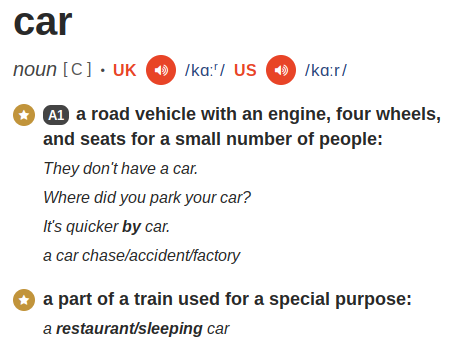
\includegraphics[width=0.37\textwidth]{ch05-cambridge-definition}
      \caption{Example of an HTML page from the Cambridge dictionary.}
      \label{fig:cambrige}
    \end{figure}

    \noindent \texttt{dict2vec} does not focus on learning a vector for each
    sense of polysemous words so the definitions of all the senses of a word are
    concatenated and considered as a single definition. For each word, its
    definitions from all the dictionaries are also concatenated. Stop words and
    punctuation are removed, words are lowercased and a pre-processing step is
    applied to transform plural words to singular ones. For the word ``car'',
    the definition obtained is:

    \begin{quote}
      \small
      \textbf{car}: road vehicle engine wheel seat small number people part
      train special purpose separate part train passenger sit part train
      carrying good animal road vehicle engine wheel seating people car part
      train abbreviation capital adequacy ratio automobile vehicle running rail
      streetcar railroad car part elevator balloon modern airship carries
      passenger freight british wheeled vehicle farm cart wagon
      literary chariot war triumph archaic cart carriage selfpropelled road
      vehicle designed carry passenger wheel powered engine modifier
      conveyance passenger freight cable car carrier airship balloon railway
      vehicle passenger sleeping car buffet car railway carriage van enclosed
      platform lift
    \end{quote}

    \noindent Among the 2.2M unique words, only 200K have a definition. Strong
    and weak pairs are generated from the downloaded definitions according to
    the rules described in~\autoref{ch05:subsec:strong-weak-pairs}, leading to
    417K strong pairs (when the number of close neighbors used to extend strong
    pairs is set to 5) and 3.9M weak pairs.

  \subsection{Training settings}
    \label{ch05:subsec:training-settings}
    \subsubsection{Training corpora}
      \label{ch05:subsubsec:training-corpora}
      \texttt{dict2vec} model is trained with the generated strong and weak
      pairs and the November 2016 English dump from Wikipedia. After removing
      all XML tags found in the Wikipedia dump and converting all words to
      lowercase (with the help of Mahoney's
      script\footnote{\url{http://mattmahoney.net/dc/textdata.html\#appendixa}}),
      the corpus is separated into 3 training files containing respectively the
      first 50M tokens, the first 200M tokens, and the full dump.
      \texttt{dict2vec} uses additional knowledge during training so it would
      not be fair to compare \texttt{dict2vec} to other common models which only
      train word embeddings with a text corpus and no additional knowledge. To
      overcome this shortcoming and have a fair comparison against other models,
      the additional information extracted from definitions is also incorporated
      into the text corpora and two versions of each text training file are
      created: one containing only text from Wikipedia (noted as ``Wikipedia''
      in~\autoref{ch05:sec:results}) and another one with text from Wikipedia
      concatenated to the extracted definitions (noted as ``Wikipedia \texttt{+}
      definitions'' in~\autoref{ch05:sec:results}).

    \subsubsection{Hyperparameters of \texttt{dict2vec}}
      \label{ch05:subsubsec:hyperparameters}
      Hyperparameters for the general settings of \texttt{dict2vec} are set to
      the ones usually found in the literature, that is: $5$ negatives samples,
      $5$ training epochs, a context window composed of $5$ words, a vector size
      of $100$ dimensions (resp. $200$ and $300$) for the 50M tokens
      training file (resp. the 200M tokens and the full dump training files) and
      words with less than $5$ occurrences are removed from the corpus. For the
      specific hyperparameters of \texttt{dict2vec}, the same tuning protocol as
      in the \texttt{word2vec} and \texttt{fasttext} papers is followed to
      provide the fairest comparison against other competitors, so every other
      hyperparameters ($\beta_{s}$, $\beta_{w}$, $n_s$, $n_w$) are tuned with a
      grid search to maximize the weighted average score on a word semantic
      similarity task. For $n_s$ and $n_w$, values from 0 to 10 with a step of 1
      have been tested. For $\beta_{s}$ and $\beta_{w}$, values from 0 to 2 with
      a step of 0.05 have been tested. The optimal hyperparameters for the
      \texttt{dict2vec} model are: $n_s = 4$, $n_w = 5$, $\beta_{s} = 0.8$ and
      $\beta_{w} = 0.45$.

  \subsection{Evaluation protocol}
    \label{ch05:subsec:evaluation-protocol}
    \subsubsection{Evaluation tasks}
      \begin{itemize}
        \item \textbf{Word semantic similarity evaluation.} \texttt{dict2vec}
          follows the standard method for this evaluation task by computing the
          Spearman's rank correlation coefficient \citep{spearman1904proof}
          between human similarity evaluation of pairs of words and the cosine
          similarity of the corresponding word vectors. This task has been
          explained in more details in
          \autoref{ch01:subsubsec:semantic-similarity} of
          \autoref{chap:preliminaries}. The following classic datasets are used:
          \begin{itemize}
            \item MC-30 \citep{miller1991contextual}
            \item MEN \citep{bruni2014multimodal}
            \item MTurk-287 \citep{radinsky2011word}
            \item MTurk-771 \citep{halawi2012large}
            \item RG-65 \citep{rubenstein1965contextual}
            \item RW \citep{luong2013better}
            \item SimVerb-3500 \citep{gerz2016simverb}
            \item WordSim-353 \citep{finkelstein2001placing}
            \item YP-130 \citep{yang2006verb}
          \end{itemize}
          The same protocol as the one used by \texttt{word2vec} and
          \texttt{fasttext} is followed: pairs containing a word which does not
          occur in the training text corpus are discarded. Since
          \texttt{dict2vec} and the competitor models are all trained on the
          same corpora, they all have the same out-of-vocabulary (OOV) rate (the
          ratio of pairs not used to compute the Spearman's rank correlation
          coefficient). Each training is repeated 3 times
          and~\autoref{ch05:tab:results-semantic} reports the average score of
          the 3 training, to minimize the effect of the neural network random
          initialization. The weighted average score (\textit{W.Average}) on all
          datasets is computed by weighting each dataset score by the number of
          pairs that are evaluated in it, in the same way
          as~\citeauthor{iacobacci2016embeddings}~\citep{iacobacci2016embeddings}.

        \item \textbf{Text classification evaluation.} This task (described in
          more details in \autoref{ch01:subsubsec:text-classification-task} in
          \autoref{chap:preliminaries}) follows the same setup as in the
          \texttt{fasttext} paper~\citep{joulin2016bag}. A neural network
          composed of a single hidden layer is trained, where the input layer
          corresponds to the Bag-of-Words of a document and the output layer is
          the probability to belong to each possible class. Weights between the
          input and the hidden layer are initialized with the learned word
          embeddings and are freezed during the neural network training so that
          the evaluation score solely depends on the word embeddings used for
          the initialization. The weights of the neural network are learned with
          the stochastic gradient descent technique to minimize the number of
          prediction errors. The datasets used for this classification task are:
          AG-News\footnote{\url{https://www.di.unipi.it/~gulli/AG_corpus_of_news_articles.html}},
          DBpedia~\citep{auer2007dbpedia} and Yelp
          reviews\footnote{\url{https://www.yelp.com/dataset}} (polarity and
          full). Each dataset is split into a training and a test file. The
          same training and test files are used for all models. The
          classification accuracy obtained on the test file is reported
          in~\autoref{ch05:tab:results-classification}.
      \end{itemize}

    \subsubsection{Baselines}
      Two other models are used to compare the performances of \texttt{dict2vec}
      against competitors:
      \texttt{word2vec}\footnote{\url{https://github.com/tmikolov/word2vec}} and
      \texttt{fasttext}\footnote{\url{https://github.com/facebookresearch/fastText}}.
      Both competitors have been trained on the same 3 corpora as
      \texttt{dict2vec} (50M tokens, 200M tokens and full Wikipedia dump) and
      their 2 respective versions (``Wikipedia'' and ``Wikipedia \texttt{+}
      definitions'' ) described in~\autoref{ch05:subsubsec:training-corpora}.
      They use the same general hyperparameters as \texttt{dict2vec}, which are
      detailed in~\autoref{ch05:subsubsec:hyperparameters} and commonly used in
      the literature. \texttt{word2vec} is trained with its Skip-gram
      architecture because the \texttt{dict2vec} method is based on the
      Skip-gram model. \texttt{GloVe} has also been trained on the same corpora
      with its respective hyperparameters described
      in~\citep{pennington2014glove} but their results are lower than all the
      other baselines (weighted averages on the word semantic similarity task
      are $0.350$ for the 50M file, $0.389$ for the 200M file and $0.454$ for
      the full dump) so the results of \texttt{GloVe} are not reported
      in~\autoref{ch05:tab:results-semantic}.\medskip

      To compare \texttt{dict2vec} against another method which uses additional
      information, word embeddings learned on the ``Wikipedia'' corpus are
      retrofitted with the method of ~\cite{faruqui2015retrofitting}.
      \texttt{retrofitting} introduces external knowledge from the WordNet
      semantic lexicon~\citep{miller1995wordnet}. Word embeddings learned with
      \texttt{dict2vec} and the other competitors are all
      retrofitted\footnote{\url{https://github.com/mfaruqui/retrofitting}} with
      the $\text{WN}_{all}$ semantic lexicon from WordNet and $10$ iterations,
      as advised in the paper of~\citeauthor{faruqui2015retrofitting}. Another
      comparison is made by evaluating the performances of \texttt{dict2vec}
      using WordNet as an additional resource instead of dictionaries.

\section{Results and model analysis}
  \label{ch05:sec:results}
  This section presents the results obtained by the word embeddings learned with
  the \texttt{dict2vec} model on two different tasks: a word semantic similarity
  task (\autoref{ch05:subsec:results-semantic}) and a text classification task
  (\autoref{ch05:subsec:results-classification}). In addition to comparing
  \texttt{dict2vec} to other common methods used to learn word vectors, a
  comparison to a method which improves the captured semantic information with
  additional external knowledge is presented
  in~\autoref{ch05:subsec:dict2vec-vs-retrofitting}. Moreover, a comparison
  between the use of dictionaries and the use of WordNet in the
  \texttt{dict2vec} architecture is presented in
  \autoref{ch05:subsec:dictionaries-vs-wordnet}. Finally,
  \autoref{ch05:subsec:d2v-hyperparameters} analyzes the influence of the
  different hyperparameters of \texttt{dict2vec}.

  \subsection{Word semantic similarity}
    \label{ch05:subsec:results-semantic}

    \autoref{ch05:tab:results-semantic} reports the Spearman's rank correlation
    scores obtained on several datasets and following the protocol described
    in~\autoref{ch05:subsec:evaluation-protocol} for the word semantic
    similarity task. Each model (\texttt{word2vec}, \texttt{fasttext} and
    \texttt{dict2vec}) have been trained on 3 different corpora sizes: 50M
    tokens, 200M tokens and the full Wikipedia dump (which contains around 4.1B
    tokens). Since all the models are trained on the same corpora, the
    percentage of out-of-vocabulary (OOV) pairs (a pair of words in a similarity
    dataset where one of the word is not in the training corpus) is the same for
    all the models. The ratio of OOV pairs for each dataset is reported
    in~\autoref{ch05:tab:oov}. All the pairs have words within the training
    corpora except for the RW dataset, which is expected because this dataset
    contains many Rare Words (RW) which are only found in large corpora (like
    the full Wikipedia dump).

    % table to compare OOV rates with different corpus sizes
    \begin{table}[h]
      \centering
      \begin{tabular}{lccc}
                    & 50M & 200M & full\\
        \toprule[0.1em]
          MC-30     & 0\% & 0\%  & 0\% \\
          MEN-TR-3k & 0\% & 0\%  & 0\% \\
          MTurk-287 & 0\% & 0\%  & 0\% \\
          MTurk-771 & 0\% & 0\%  & 0\% \\
          RG-65     & 0\% & 0\%  & 0\% \\
          RW        & 36\%& 16\% & 2\% \\
          SimVerb   & 3\% & 0\%  & 0\% \\
          WS353-ALL & 0\% & 0\%  & 0\% \\
          WS353-REL & 0\% & 0\%  & 0\% \\
          WS353-SIM & 0\% & 0\%  & 0\% \\
          YP-130    & 3\% & 0\%  & 0\% \\
        \bottomrule[0.1em]
      \end{tabular}
      \caption[Percentage of pairs of words not evaluated in the semantic
      similary task.]{Percentage of pairs of words not used for evaluation in
      the semantic similarity task for different sizes of corpus files and
      datasets. When a pair contains a word not in the vocabulary of the corpus,
      it is discarded for the evaluation.}
      \label{ch05:tab:oov}
    \end{table}

    % Table of word semantic similarity scores
    \begin{table}
      \begin{subtable}{\textwidth} % 50M corpus
        \centering
        % 8 columns (1 + 3 + 1 + 3):
        %   - dataset
        %   - 3 models on Wikipedia
        %   - 1 blank column
        %   - 3 models on Wikipedia+definitions
        \resizebox{0.88\textwidth}{!}{
        \begin{tabular}{@{}lccccccc@{}}
          & \multicolumn{3}{c}{Wikipedia} &&
            \multicolumn{3}{c}{Wikipedia \texttt{+} definitions}\\
          % \cmidrule command of booktabs allows for an optional argument using
          % parentheses ( ) to specify on which side it should be reduced.
          \cmidrule(lr){2-4} \cmidrule(l){6-8}
          & \texttt{word2vec} & \texttt{fasttext} & \texttt{dict2vec} &
          & \texttt{word2vec} & \texttt{fasttext} & \texttt{dict2vec}\\
          \midrule[0.1em]
            %                     w2v     FT       our
            MC-30              & 0.697 & 0.722 & 0.840 &
                               & 0.847 & 0.823 & \bf{0.859}\\
            MEN-TR-3k          & 0.692 & 0.697 & 0.733 &
                               & 0.753 & \bf{0.767} & 0.762\\
            MTurk-287          & 0.657 & 0.657 & 0.665 &
                               & \bf{0.688} & 0.685 & 0.682\\
            MTurk-771          & 0.596 & 0.597 & 0.685 &
                               & 0.677 & 0.692 & \bf{0.713}\\
            RG-65              & 0.714 & 0.671 & 0.824 &
                               & 0.865 & 0.842 & \bf{0.875}\\
            RW                 & 0.375 & 0.442 & 0.475 &
                               & 0.420 & \bf{0.512} & 0.489\\
            SimVerb            & 0.165 & 0.179 & 0.363 &
                               & 0.371 & 0.374 & \bf{0.432}\\
            WS353-ALL          & 0.660 & 0.657 & 0.738 &
                               & 0.739 & 0.739 & \bf{0.753}\\
            WS353-REL          & 0.619 & 0.623 & 0.679 &
                               & \bf{0.700} & 0.696 & 0.688\\
            WS353-SIM          & 0.714 & 0.714 & 0.774 &
                               & \bf{0.797} & 0.790 & 0.784\\
            YP-130             & 0.458 & 0.415 & 0.666 &
                               & 0.679 & 0.674 & \bf{0.696}\\
            \cmidrule(l){2-8}
            \textit{W.Average} & 0.453 & 0.467 & 0.564 &
                               & 0.562 & 0.582 & \bf{0.599}\\
          \bottomrule[0.1em]
        \end{tabular}}
        \caption{Trained with a Wikipedia corpus file of 50M tokens.}
        \vspace*{1em} % to add vertical space between subtables
      \end{subtable}
      \begin{subtable}{\textwidth} % 200M corpus
        \centering
        \resizebox{0.88\textwidth}{!}{
        \begin{tabular}{@{}lccccccc@{}}
          & \multicolumn{3}{c}{Wikipedia} &&
            \multicolumn{3}{c}{Wikipedia \texttt{+} definitions}\\
          \cmidrule(lr){2-4} \cmidrule(l){6-8}
          & \texttt{word2vec} & \texttt{fasttext} & \texttt{dict2vec} &
          & \texttt{word2vec} & \texttt{fasttext} & \texttt{dict2vec}\\
          \midrule[0.1em]
            %                     w2v     FT         our
            MC-30              & 0.742 & 0.795 & \bf{0.854} &
                               & 0.830 & 0.814 & 0.827\\
            MEN-TR-3k          & 0.734 & 0.754 & 0.752 &
                               & 0.758 & \bf{0.772} & 0.768\\
            MTurk-287          & 0.642 & 0.671 & 0.667 &
                               & \bf{0.671} & 0.661 & 0.666\\
            MTurk-771          & 0.628 & 0.632 & 0.682 &
                               & 0.669 & 0.675 & \bf{0.704}\\
            RG-65              & 0.771 & 0.755 & 0.857 &
                               & 0.842 & 0.829 & \bf{0.877}\\
            RW                 & 0.377 & 0.475 & 0.467 &
                               & 0.408 & \bf{0.507} & 0.478\\
            SimVerb            & 0.183 & 0.206 & 0.377 &
                               & 0.306 & 0.329 & \bf{0.424}\\
            WS353-ALL          & 0.694 & 0.701 & \bf{0.762} &
                               & 0.734 & 0.735 & 0.758\\
            WS353-REL          & 0.665 & 0.644 & \bf{0.710} &
                               & 0.706 & 0.685 & 0.699\\
            WS353-SIM          & 0.743 & 0.758 & 0.784 &
                               & \bf{0.792} & 0.792 & 0.787\\
            YP-130             & 0.449 & 0.509 & 0.616 &
                               & 0.592 & 0.639 & \bf{0.665}\\
            \cmidrule{2-8}
            \textit{W.Average} & 0.471 & 0.503 & 0.569 &
                               & 0.533 & 0.563 & \bf{0.592}\\
          \bottomrule[0.1em]
        \end{tabular}}
        \caption{Trained with a Wikipedia corpus file of 200M tokens.}
        \vspace*{1em}
      \end{subtable}
      \begin{subtable}{\textwidth} % full dump
        \centering
        \resizebox{0.88\textwidth}{!}{
        \begin{tabular}{@{}lccccccc@{}}
          & \multicolumn{3}{c}{Wikipedia} &&
            \multicolumn{3}{c}{Wikipedia \texttt{+} definitions}\\
          \cmidrule(lr){2-4} \cmidrule(l){6-8}
          & \texttt{word2vec} & \texttt{fasttext} & \texttt{dict2vec} &
          & \texttt{word2vec} & \texttt{fasttext} & \texttt{dict2vec}\\
          \midrule[0.1em]
            %                     w2v     FT         our
            MC-30              & 0.809 & 0.831 & \bf{0.860} &
                               & 0.826 & 0.815 & 0.847 \\
            MEN-TR-3k          & 0.733 & 0.752 & \bf{0.756} &
                               & 0.728 & 0.751 & 0.755 \\
            MTurk-287          & 0.660 & \bf{0.672} & 0.661 &
                               & 0.656 & 0.671 & 0.660 \\
            MTurk-771          & 0.623 & 0.631 & \bf{0.696} &
                               & 0.620 & 0.638 & 0.694 \\
            RG-65              & 0.787 & 0.817 & \bf{0.875} &
                               & 0.802 & 0.820 & 0.867 \\
            RW                 & 0.407 & 0.464 & \bf{0.482} &
                               & 0.427 & 0.468 & 0.476 \\
            SimVerb            & 0.186 & 0.222 & \bf{0.384} &
                               & 0.214 & 0.233 & 0.379 \\
            WS353-ALL          & 0.705 & 0.729 & 0.756 &
                               & 0.721 & 0.723 & \bf{0.758} \\
            WS353-REL          & 0.664 & 0.687 & 0.702 &
                               & 0.681 & 0.686 & \bf{0.703} \\
            WS353-SIM          & 0.757 & 0.775 & 0.781 &
                               & 0.767 & 0.779 & \bf{0.781} \\
            YP-130             & 0.502 & 0.533 & \bf{0.646} &
                               & 0.475 & 0.553 & 0.607 \\
            \cmidrule{2-8}
            \textit{W.Average} & 0.476 & 0.508 & \bf{0.573} &
                               & 0.488 & 0.512 & 0.570 \\
          \bottomrule[0.1em]
        \end{tabular}}
        \caption{Trained with the full Wikipedia corpus file.}
      \end{subtable}
      \caption[Evaluation of \texttt{dict2vec} and other models on a semantic
      similarity task.]{Semantic similarity scores on several datasets and
      different sizes of corpora for \texttt{word2vec}, \texttt{fasttext} and
      \texttt{dict2vec}. Each model is trained and evaluated 3 times; the mean
      score of the 3 runs is reported in the table. \textit{W.average} is the
      weighted average for all word similarity datasets.}
      \label{ch05:tab:results-semantic}
    \end{table}

    \paragraph{\texttt{dict2vec} vs. others.}
      The \texttt{dict2vec} model outperforms other approaches on most of the
      datasets for the 50M and the 200M tokens files, and on all datasets
      (excepted one) for the full Wikipedia dump (this is significant according
      to a two-sided Wilcoxon signed-rank test with $\alpha=0.05$). On the
      weighted average score, the \texttt{dict2vec} model improves
      \texttt{fasttext} performances on the ``Wikipedia'' corpus by $20.8\%$ for
      the 50M tokens file, by $13.1\%$ for the 200M tokens file and by $12.8\%$
      for the full dump. Even when \texttt{fasttext} has access to additional
      knowledge during training (scores in the column ``Wikipedia \texttt{+}
      definitions''), the \texttt{dict2vec} model still has better performances
      with an increase of $2.9\%$ for the 50M tokens file, $5.2\%$ for the 200M
      tokens file and $11.3\%$ for the full dump.

      Models based on external knowledge sources presented
      in~\autoref{ch03:sec:external-resources} of~\autoref{chap:methods-we} do
      not provide word semantic similarity scores for all the datasets used in
      this evaluation. However, for the reported scores, \texttt{dict2vec}
      outperforms these
      models:~\citeauthor{kiela2015specializing}~\citep{kiela2015specializing}
      reach a score of $0.72$ on the MEN dataset ($0.756$ for
      \texttt{dict2vec});~\citeauthor{xu2014rc}~\citep{xu2014rc} obtain $0.683$
      on the WS353-ALL dataset ($0.758$ for \texttt{dict2vec}).

    \paragraph{Adding definitions to the corpus.}
      The column ``Wikipedia \texttt{+} definitions''
      in~\autoref{ch05:tab:results-semantic}, which represents the case where
      training corpora are composed of Wikipedia and word definitions
      concatenated to them, has better results than the column ``Wikipedia''
      which represents training corpora only composed of Wikipedia: $+18.3\%$ on
      average for the 50M tokens file, $+9.7\%$ for the 200M tokens file. This
      demonstrates the strong semantic relations one can find in definitions and
      that simply incorporating definitions into small training corpora can
      boost the performances of the word embeddings trained on them. This is
      significant because the training time is largely decreased when the corpus
      file is smaller (training with the 50M tokens corpus file is 150 times
      faster than training on the full Wikipedia corpus) so adding definitions
      is a better option than extending the corpus with content from Wikipedia.
      However, when the training file is large (full dump), the supervision
      brought by strong and weak pairs is more efficient to improve the word
      semantic similarity scores than adding word definitions to the corpus as
      the boost brought by the concatenation of definitions is not significant
      for the full dump ($+0.9\%$ on average). It is also important to observe
      that, although the \texttt{dict2vec} model is superior for each corpus
      size, its word embeddings trained on the ``Wikipedia'' corpus of 50M
      tokens outperforms the word embeddings of other models trained on the
      ``Wikipedia'' full dump (an improvement of $11\%$ compared to the results
      of \texttt{fasttext} vectors, its best competitor, trained on the full
      dump). This means that considering strong and weak pairs in a model is
      more efficient than increasing the training corpus size and that using
      dictionaries is a good way to improve the quality of the embeddings when
      the training file is small.

  \subsection{Text classification accuracy}
    \label{ch05:subsec:results-classification}

    % Table of text classification scores
    \begin{table}[!t]
      \begin{subtable}{\textwidth}
        \centering
        \resizebox{0.85\textwidth}{!}{
        \begin{tabular}{@{}lccccccc@{}}
          & \multicolumn{3}{c}{Wikipedia} &&
            \multicolumn{3}{c}{Wikipedia \texttt{+} definitions}\\
          \cmidrule(lr){2-4} \cmidrule(l){6-8}
          & \texttt{word2vec} & \texttt{fasttext} & \texttt{dict2vec} &
          & \texttt{word2vec} & \texttt{fasttext} & \texttt{dict2vec}\\
          \midrule[0.1em]
            %            w2v     FT         our
            AG-News   & \bf{87.4} & 86.8 & 87.1 &
                      & 87.1 & 87.1 & 86.6\\
            DBPedia   & 93.5 & 94.2 & \bf{94.4} &
                      & 94.2 & 94.4 & 94.4\\
            Yelp Pol. & 80.8 & 82.1 & 83.2 &
                      & 83.5 & \bf{84.2} & 83.4\\
            Yelp Full & 45.1 & 46.0 & 47.1 &
                      & 46.9 & \bf{47.3} & 47.2\\
          \bottomrule[0.1em]
        \end{tabular}}
        \caption{Trained with a Wikipedia corpus file of 50M tokens.}
        \vspace*{1em}
      \end{subtable}
      \begin{subtable}{\textwidth}
        \centering
        \resizebox{0.85\textwidth}{!}{
        \begin{tabular}{@{}lccccccc@{}}
          & \multicolumn{3}{c}{Wikipedia} &&
            \multicolumn{3}{c}{Wikipedia \texttt{+} definitions}\\
          \cmidrule(lr){2-4} \cmidrule(l){6-8}
          & \texttt{word2vec} & \texttt{fasttext} & \texttt{dict2vec} &
          & \texttt{word2vec} & \texttt{fasttext} & \texttt{dict2vec}\\
          \midrule[0.1em]
            %            w2v     FT         our
            AG-News   & \bf{88.6} & 88.0 & 88.0 &
                      & 88.2 & 88.1 & 88.0\\
            DBPedia   & 95.2 & 95.7 & \bf{96.0} &
                      & 95.6 & 95.8 & 95.9\\
            Yelp Pol. & 83.7 & 85.2 & 85.6 &
                      & 85.5 & 85.9 & \bf{85.9}\\
            Yelp Full & 47.7 & 48.8 & 49.9 &
                      & 49.1 & 49.5 &\bf{50.1}\\
          \bottomrule[0.1em]
        \end{tabular}}
        \caption{Trained with a Wikipedia corpus file of 200M tokens.}
        \vspace*{1em}
      \end{subtable}
      \begin{subtable}{\textwidth}
        \centering
        \resizebox{0.85\textwidth}{!}{
        \begin{tabular}{@{}lccccccc@{}}
          & \multicolumn{3}{c}{Wikipedia} &&
            \multicolumn{3}{c}{Wikipedia \texttt{+} definitions}\\
          \cmidrule(lr){2-4} \cmidrule(l){6-8}
          & \texttt{word2vec} & \texttt{fasttext} & \texttt{dict2vec} &
          & \texttt{word2vec} & \texttt{fasttext} & \texttt{dict2vec}\\
          \midrule[0.1em]
            %            w2v     FT         our
            AG-News   & 88.5 & \bf{88.7} & 88.1 &
                      & 88.5 & 88.7 & 88.4\\
            DBPedia   & 96.6 & 96.7 & 96.8 &
                      & 96.6 & 96.7 & \bf{96.9}\\
            Yelp Pol. & 86.5 & 87.2 & \bf{87.6} &
                      & 86.7 & 87.4 & 87.5\\
            Yelp Full & 50.6 & 51.2 & 51.6 &
                      & 50.6 & 51.4 & \bf{51.8}\\
          \bottomrule[0.1em]
        \end{tabular}}
        \caption{Trained with the full Wikipedia corpus file.}
      \end{subtable}
      \caption[Evaluation of \texttt{dict2vec} and other models on a text
      classification task.]{Accuracies on a text classification task (percentage
      of correctly classified documents). Each model is trained and evaluated 3
      times; the mean score of the 3 runs is reported.}
      \label{ch05:tab:results-classification}
    \end{table}

    \autoref{ch05:tab:results-classification} reports the classification
    accuracies (percentage of correctly classified documents) obtained for
    \texttt{word2vec}, \texttt{fasttext} and \texttt{dict2vec} on the datasets
    listed in~\autoref{ch05:subsec:evaluation-protocol}. The \texttt{dict2vec}
    model achieves similar level of performances as \texttt{word2vec} and
    \texttt{fasttext} when trained on the 50M tokens file and slightly better
    results when trained on the 200M tokens file and on the full dump. Using
    strong and weak pairs as a supervision during training does not make the
    \texttt{dict2vec} model specialized for the word semantic similarity task,
    which demonstrates that the learned embeddings can also be used in
    downstream models for extrinsic tasks. In this classification evaluation,
    values of the embeddings are not updated during the training
    phase (only the parameters of the classifier are learned)
    since the objective is to evaluate the capacity of the embeddings to be used
    in another task rather than obtaining the best possible classification
    model. It is however possible to obtain better results than those presented
    in~\autoref{ch05:tab:results-classification} by updating the embeddings
    values during training with the supervised information of labeled documents
    in order to adapt the embeddings for this classification task, as done
    by~\citeauthor{joulin2016bag}~\citep{joulin2016bag}.

  \subsection{\texttt{dict2vec} vs. \texttt{retrofitting}}
    \label{ch05:subsec:dict2vec-vs-retrofitting}

    % Table to compare the score of retrofitted vectors and original d2v vectors
    \begin{table}[h]
      \centering
      \resizebox{\textwidth}{!}{
        \begin{tabular}{@{}lcccccccccccc@{}} % all 13 columns are centered,
                                             % except 1st one that left aligned
        &
        & \multicolumn{3}{c}{50M} & \phantom{}
        & \multicolumn{3}{c}{200M} & \phantom{}
        & \multicolumn{3}{c}{full}\\
        \cmidrule{3-5} \cmidrule{7-9} \cmidrule{11-13}
          && \texttt{w2v}\indic{rf} & \texttt{ft}\indic{rf} & \texttt{d2v}\indic{rf}
          && \texttt{w2v}\indic{rf} & \texttt{ft}\indic{rf} & \texttt{d2v}\indic{rf}
          && \texttt{w2v}\indic{rf} & \texttt{ft}\indic{rf} & \texttt{d2v}\indic{rf}\\
        \midrule[0.1em]
        %    w2v           FT         d2v
        \multirow{2}{*}{MC-30}
          &vs. self (not \teal{rf}) &
                +13.9\% &      +9.2\% & +1.3\% &&
                 +5.8\% &      +4.8\% & +3.0\% &&
                 +5.2\% &      +2.9\% & +1.2\% \\
          &vs. \texttt{d2v} (not \teal{rf}) &
            \bf{-7.3\%} & \bf{-4.4\%} &    $-$ &&
            \bf{-3.6\%} & \bf{-2.4\%} &    $-$ &&
            \bf{-1.0\%} & \bf{-0.6\%} &    $-$ \\
        \cmidrule{2-13}
        \multirow{2}{*}{MEN-TR-3k}
          &vs. self (not \teal{rf}) &
                 +0.9\% &      -0.7\% & -0.1\% &&
                 +0.7\% &      -1.9\% & +0.4\% &&
                 +1.4\% &      -2.8\% & +1.6\% \\
          &vs. \texttt{d2v} (not \teal{rf}) &
            \bf{-4.2\%} & \bf{-7.4\%} &    $-$ &&
            \bf{-1.3\%} & \bf{-1.6\%} &    $-$ &&
            \bf{-1.7\%} & \bf{-3.3\%} &    $-$ \\
        \cmidrule{2-13}
        \multirow{2}{*}{MTurk-287}
          &vs. self (not \teal{rf}) &
                 +1.4\% &      +0.2\% & +3.5\% &&
                 -2.9\% &      -3.3\% & +3.0\% &&
                 -0.9\% &      -5.7\% & +1.1\% \\
          &vs. \texttt{d2v} (not \teal{rf}) &
            \bf{-1.2\%} & \bf{-4.0\%} &    $-$ &&
            \bf{-4.3\%} & \bf{-2.7\%} &    $-$ &&
            \bf{-1.1\%} & \bf{-4.1\%} &    $-$ \\
        \cmidrule{2-13}
        \multirow{2}{*}{MTurk-771}
          &vs. self (not \teal{rf}) &
                 +8.2\% &      +4.9\% & +1.6\% &&
                 +6.3\% &      +4.3\% & +1.5\% &&
                 +4.5\% &      +1.6\% & +0.6\% \\
          &vs. \texttt{d2v} (not \teal{rf}) &
            \bf{-7.3\%} & \bf{-8.8\%} &    $-$ &&
            \bf{-3.8\%} & \bf{-3.4\%} &    $-$ &&
            \bf{-6.5\%} & \bf{-7.9\%} &    $-$ \\
        \cmidrule{2-13}
        \multirow{2}{*}{RG-65}
          &vs. self (not \teal{rf}) &
                +10.9\% &     +17.1\% & +4.0\% &&
                 +6.6\% &      +8.5\% & +3.0\% &&
                 +7.0\% &      +5.0\% & +2.4\% \\
          &vs. \texttt{d2v} (not \teal{rf}) &
            \bf{-2.1\%} & \bf{-4.9\%} &    $-$ &&
            \bf{-2.2\%} & \bf{-4.4\%} &    $-$ &&
            \bf{-3.8\%} & \bf{-1.9\%} &    $-$ \\
        \cmidrule{2-13}
        \multirow{2}{*}{RW}
          &vs. self (not \teal{rf}) &
                 -20.3\% &    -24.4\% & -14.3\% &&
                 -24.4\% &    -25.9\% & -20.3\% &&
                 -18.7\% &    -25.4\% & -19.1\% \\
          &vs. \texttt{d2v} (not \teal{rf}) &
            \bf{-37.4\%} & \bf{-26.9\%} &   $-$ &&
            \bf{-37.7\%} & \bf{-24.6\%} &   $-$ &&
            \bf{-31.3\%} & \bf{-28.2\%} &   $-$ \\
        \cmidrule{2-13}
        \multirow{2}{*}{Simverb}
          &vs. self (not \teal{rf}) &
                 +46.0\% &      +34.0\% & +19.8\% &&
                 +49.7\% &      +39.8\% & +19.9\% &&
                 +44.6\% &      +38.7\% & +16.7\% \\
          &vs. \texttt{d2v} (not \teal{rf}) &
            \bf{-34.4\%} & \bf{-28.4\%} &     $-$ &&
            \bf{-30.5\%} & \bf{-23.6\%} &     $-$ &&
            \bf{-29.9\%} & \bf{-19.8\%} &     $-$ \\
        \cmidrule{2-13}
        \multirow{2}{*}{WS353-ALL}
          &vs. self (not \teal{rf}) &
                  -4.2\% &     -10.8\% & -1.1\% &&
                  -3.2\% &      -8.0\% & -1.3\% &&
                  -4.4\% &     -10.7\% & -2.0\% \\
          &vs. \texttt{d2v} (not \teal{rf}) &
            \bf{-13.8\%} &\bf{-19.2\%} &    $-$ &&
            \bf{-11.9\%} &\bf{-15.4\%} &    $-$ &&
            \bf{-10.8\%} &\bf{-13.9\%} &    $-$ \\
        \cmidrule{2-13}
        \multirow{2}{*}{WS353-REL}
          &vs. self (not \teal{rf}) &
                 -16.1\% &     -22.7\% & -4.9\% &&
                 -10.4\% &     -17.9\% & -4.5\% &&
                 -10.7\% &     -19.7\% & -6.0\% \\
          &vs. \texttt{d2v} (not \teal{rf}) &
            \bf{-20.9\%} &\bf{-27.2\%} &    $-$ &&
            \bf{-17.7\%} &\bf{-25.5\%} &    $-$ &&
            \bf{-15.5\%} &\bf{-21.4\%} &    $-$ \\
        \cmidrule{2-13}
        \multirow{2}{*}{WS353-SIM}
          &vs. self (not \teal{rf}) &
                 +4.3\% &      +0.8\% & +3.2\% &&
                 +2.6\% &      +0.0\% & +3.2\% &&
                 +0.0\% &      -3.6\% & +2.4\% \\
          &vs. \texttt{d2v} (not \teal{rf}) &
            \bf{-3.9\%} & \bf{-6.7\%} &    $-$ &&
            \bf{-2.9\%} & \bf{-3.3\%} &    $-$ &&
            \bf{-3.0\%} & \bf{-4.4\%} &    $-$ \\
        \cmidrule{2-13}
        \multirow{2}{*}{YP-130}
          &vs. self (not \teal{rf}) &
                 +17.8\% &      +3.2\% & +3.3\% &&
                 +13.0\% &      +6.9\% & +8.0\% &&
                 +11.1\% &      +8.3\% & +5.0\% \\
          &vs. \texttt{d2v} (not \teal{rf}) &
            \bf{-23.6\%} &\bf{-28.2\%} &    $-$ &&
            \bf{-16.6\%} &\bf{-11.7\%} &    $-$ &&
            \bf{-13.6\%} &\bf{-10.7\%} &    $-$ \\
        \bottomrule[0.15em]
      \end{tabular}}
      \caption[Semantic similarity scores differences between
      \texttt{retrofitting} and \texttt{dict2vec}.]{(\teal{rf} = retrofitted).
      Percentage differences of word semantic similarity scores between
      retrofitted vectors (\texttt{X}\indic{rf}) and non-retrofitted vectors
      (not \teal{rf}).  Each model is compared to their own non-retrofitted
      version (vs. self) and \texttt{dict2vec} non-retrofitted version (vs.
      \texttt{d2v}). A positive (resp.  negative) percentage indicates that
      \texttt{retrofitting} improves (resp.  deteriorates) the semantic score
      compared to non-retrofitted vectors.  As an illustration: the top left
      value $+13.9\%$ means that \texttt{word2vec} retrofitted vectors improves
      the initial \texttt{word2vec} vectors performance by $13.9\%$, while the
      value $-7.3\%$ right below it means that their performance is
      $7.3\%$ lower than the non-retrofitted vectors of \texttt{dict2vec}.}
      \label{ch05:tab:results-faruqui}
    \end{table}

    \texttt{retrofitting} \citep{faruqui2015retrofitting} is a method to improve
    the semantic information encoded into word embeddings \textbf{after} they
    have been trained on a corpus (this method is described in more details
    in~\autoref{ch03:sec:external-resources} of~\autoref{chap:methods-we}).
    \citeauthor{faruqui2015retrofitting} method has been applied on each of the
    word embeddings trained on ``Wikipedia'' corpora with pairs of related words
    extracted from WordNet to produce retrofitted vectors of the
    \texttt{word2vec}, \texttt{fasttext} and \texttt{dict2vec} models.
    Retrofitted vectors have been evaluated on the word semantic similarity task
    on all the datatsets and scores of retrofitted vectors are compared to
    either: (i) the score of non-retrofitted vectors for the same model and the
    same corpus size (vs. self (not \teal{rf})); (ii) the score of
    non-retrofitted vectors of \texttt{dict2vec} for the same corpus size (vs.
    \texttt{d2v} (not \teal{rf})). The percentages of score differences are
    reported in~\autoref{ch05:tab:results-faruqui}.\smallskip
    % using a \medskip here fucks up the formatting

    The \texttt{retrofitting} method improves the word semantic similarity
    scores for all models on almost all datasets because the percentages
    differences are almost always positive when retrofitted vectors are compared
    to their non-retrofitted version (``vs. self (not \teal{rf})''
    in~\autoref{ch05:tab:results-faruqui}). However, for the datasets RW,
    WS353-ALL and WS353-REL, the percentages are negative, which indicates that
    \texttt{retrofitting} deteriorates the semantic linguistic information
    encoded into the word embeddings which is needed to evaluate that pairs from
    those datasets are related. While \texttt{retrofitting} can improve the
    quality of information encoded into word embeddings and thus increase the
    scores on the semantic similarity task, it cannot reach the performance
    increase that \texttt{dict2vec} brings. Indeed, even when \texttt{word2vec}
    and \texttt{fasttext} vectors are retrofitted (columns
    \texttt{w2v}\indic{rf} and \texttt{ft}\indic{rf}
    in~\autoref{ch05:tab:results-faruqui}), their scores are still lower than
    the scores of non-retrofitted \texttt{dict2vec} vectors (every percentages
    in the ``vs. \texttt{d2v} (not \teal{rf})'' rows are negative). It can also
    be noticed that \texttt{dict2vec} model is compatible with a retrofitting
    improvement method as its scores are also increased with
    the~\citeauthor{faruqui2015retrofitting} method. \texttt{dict2vec} uses
    additional information from dictionaries while \texttt{retrofitting} uses
    information from WordNet. This demonstrates that the two external sources of
    kwowledge are not overlapping nor exclusive and that a model using both have
    better performances than a model which uses only one of the two.

  \subsection{Dictionaries vs. WordNet}
    \label{ch05:subsec:dictionaries-vs-wordnet}
    \autoref{tab:retrofit-wordnet-dict} reports the weighted average of semantic
    similarity scores of vectors obtained after training (not retrofitted) and
    vectors retrofitted with either pairs from WordNet or pairs generated from
    dictionaries.  Retrofitting with dictionaries pairs outperforms retrofitting
    with WordNet pairs, meaning that information from dictionaries is better
    suited to improve word embeddings towards semantic similarities when
    retrofitting.

    % table to compare retrofitting w/ wordnet vs retrofitting w/ dictionaries
    \begin{table}[h!]
      \centering
      %\small
      \begin{tabular}{ccccc}
        & & not retrofitted & $\text{retrofitted}_{\text{WordNet}}$
                            & $\text{retrofitted}_{\text{dictionaries}}$ \\
        \toprule
        \multirow{3}{*}{50M}
          & \texttt{word2vec} & 0.453 & 0.474 & \bf{0.479} \\
          & \texttt{fasttext} & 0.467 & 0.476 & \bf{0.489} \\
          & \texttt{dict2vec} & 0.569 & 0.582 & \bf{0.582} \\
        \midrule
        \multirow{3}{*}{200M}
          & \texttt{word2vec} & 0.471 & 0.488 & \bf{0.494} \\
          & \texttt{fasttext} & 0.503 & 0.504 & \bf{0.524} \\
          & \texttt{dict2vec} & 0.569 & 0.581 & \bf{0.587} \\
        \midrule
        \multirow{3}{*}{full}
          & \texttt{word2vec} & 0.488 & 0.507 & \bf{0.512} \\
          & \texttt{fasttext} & 0.508 & 0.503 & \bf{0.529} \\
          & \texttt{dict2vec} & 0.571 & 0.583 & \bf{0.592} \\
        \bottomrule
      \end{tabular}
      \caption[Semantic similarity scores when retrofitting with WordNet or
      dictionaries.]{Weighted average of word semantic similarity scores for
      non-retrofitted vectors and after retrofitting vectors with
      WordNet pairs or with dictionary pairs.}
      \label{tab:retrofit-wordnet-dict}
    \end{table}

    To compare the linguistic information one can found in WordNet or in
    dictionaries, the \texttt{dict2vec} model has also been trained without
    using any strong nor weaks pairs during training or by using WordNet pairs
    as strong pairs. When no pairs are used, the \texttt{dict2vec} model is
    equivalent to the \texttt{word2vec} Skip-gram model. Weighted average of
    word semantic scores are reported
    in~\autoref{ch05:tab:training-wordnet-dict}. Training with WordNet pairs
    used as strong pairs increases the scores compared to a model that does not
    use any pairs at all, showing that the supervision brought by the positive
    sampling of \texttt{dict2vec} is beneficial to the model. But it is not as
    good as when the model uses dictionary pairs, demonstrating once again that
    dictionaries contain more semantic information than WordNet.

    % table to compare dict2vec using wordnet pairs vs. dictionary pairs
    \begin{table}[htb]
      \centering
      \begin{tabular}{cccc}
                              &  50M  &  200M & full \\
        \toprule
        No pairs              & 0.453 & 0.471 & 0.488 \\
        With WordNet pairs    & 0.564 & 0.566 & 0.559 \\
        With dictionary pairs & \bf{0.569} & \bf{0.569} & \bf{0.571} \\
        \bottomrule
      \end{tabular}
      \caption[Semantic similarity scores when using pairs from WordNet or
      dictionaries.]{Weighted average semantic similarity scores of
      \texttt{dict2vec} models when trained without pairs and with WordNet or
      dictionary pairs.}
      \label{ch05:tab:training-wordnet-dict}
    \end{table}

  \subsection{Influence of \texttt{dict2vec} hyperparameters}
    \label{ch05:subsec:d2v-hyperparameters}
    \paragraph{Number of strong and weak pairs.}
      The different experiments carried out when training the \texttt{dict2vec}
      model has shown one thing: the number of strong and weak pairs (resp.
      $n_s$ and $n_w$) drawn for each word must be set accordingly to the size
      of the training file. For the 50M and the 200M tokens files, the
      \texttt{dict2vec} model is set with the hyperparameters $n_s = 4$ and $n_w
      = 5$. When training on the full dump (which is 20 times larger than the
      200M tokens file because it contains about 4.1B tokens), the number of
      context windows in the corpus is largely increased, so is the number of
      ($target,~context$) pairs and thus the number of times the positive
      sampling is used for the most frequent words. Therefore, the influence of
      strong and weak pairs needs to be adjusted and decreased because frequent
      words would be learned mainly from their strong and weak pairs not from
      the context windows in which they occur. When trained on the full dump,
      the number of strong and weak pairs used to learn word embeddings are set
      to $n_s = 2$ and $n_w = 3$.

    \paragraph{Weight of strong and weak pairs.}
      For the hyperparameters of the positive sampling, an empirical grid search
      shows that a $\frac{1}{2}$ ratio between $\beta_s$ and $\beta_w$ is a good
      rule-of-thumb for tuning these hyperparameters. It has also been noticed
      that when these coefficients are too low ($\beta_s \leq 0.5$ and $\beta_w
      \leq 0.2$), results get worse because the model does not take into account
      the information from the strong and weak pairs. On the other side, when
      they are too high ($\beta_s \geq 1.2$ and $\beta_w \geq 0.6$), the model
      discards too much information from the context in favor of the information
      from the pairs. This behavior is similar when the number of strong and
      weak pairs is too low or too high ($n_s, n_w \leq 2$ or $n_s, n_w \geq
      5$).

    \paragraph{Number of negative samples.}
      The controlled negative sampling of \texttt{dict2vec} (see
      \autoref{ch05:subsec:controlled-negative-sampling}), which prevents the
      vectors of words forming a strong or a weak pair to be moved apart when
      words are randomly chosen during the negative sampling, increases the
      weighted average semantic similarity scores of learned word embeddings by
      $0.7\%$ compared to the non-controlled version. Increasing the number of
      negative samples used during the training phase does not significantly
      improve the results except on the RW dataset where using 25 negative
      samples can boost the scores by $10\%$, as shown
      in~\autoref{ch05:fig:negative-sampling}. Indeed, this dataset is mostly
      composed of rare words so word embeddings must learn to differentiate
      unrelated words rather than learning which vectors should be moved closer.

      % figure to show evolution of score when number of negative samples change
      \begin{figure}[h]
        \centering
          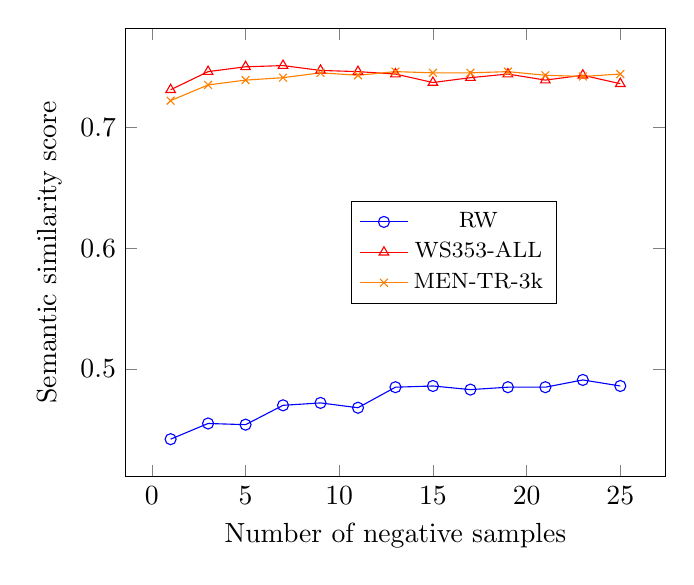
\begin{tikzpicture}
          \begin{axis}[
              xlabel=Number of negative samples,
              ylabel=Semantic similarity score,
              legend style={at={(0.8,0.5)}, anchor=east, font=\footnotesize}]
            \addplot[color=blue, mark=o] coordinates { % RW-STANFORD
              (1,0.442)
              (3,0.455)
              (5,0.454)
              (7,0.470)
              (9,0.472)
              (11,0.468)
              (13,0.485)
              (15,0.486)
              (17,0.483)
              (19,0.485)
              (21,0.485)
              (23,0.491)
              (25,0.486)
            };
            \addplot[color=red, mark=triangle] coordinates { % WS-353-ALL
              (1,0.731)
              (3,0.746)
              (5,0.750)
              (7,0.751)
              (9,0.747)
              (11,0.746)
              (13,0.744)
              (15,0.737)
              (17,0.741)
              (19,0.744)
              (21,0.739)
              (23,0.743)
              (25,0.736)
            };
            \addplot[color=orange, mark=x] coordinates { % MEN
              (1,0.722)
              (3,0.735)
              (5,0.739)
              (7,0.741)
              (9,0.745)
              (11,0.743)
              (13,0.746)
              (15,0.745)
              (17,0.745)
              (19,0.746)
              (21,0.743)
              (23,0.742)
              (25,0.744)
            };
            \legend{RW, WS353-ALL, MEN-TR-3k}
          \end{axis}
        \end{tikzpicture}
        \caption[Evolution of semantic similarity according to the number of
        negative samples.]{Semantic similarity scores on several datasets (RW,
        WS353-ALL and MEN-TR-3k) when the \texttt{dict2vec} model is trained
        with different numbers of negative samples.}
        \label{ch05:fig:negative-sampling}
      \end{figure}

    \paragraph{Dimensions of word embeddings.}
      Word embeddings with different numbers of dimensions have been trained
      with the \texttt{fasttext} and \texttt{dict2vec} models on the
      ``Wikipedia'' corpus of 50M tokens. Their semantic similarity scores on RW
      and WS353-ALL datasets are reported
      in~\autoref{ch05:fig:dimensions-embeddings}. It can be observed that
      \texttt{dict2vec} is still able to outperform the competitor approach when
      the number of dimensions of vectors is reduced to $20$ or $40$. Moreover,
      increasing the number of dimensions does increase the scores but only up
      to a certain point. When the number of dimensions is higher than 100, no
      significant improvements in semantic similarity scores are observed, which
      supports the fact that other common approaches choose vectors of dimension
      100 when the training corpus is small.

      \begin{figure}[h]
        \centering
          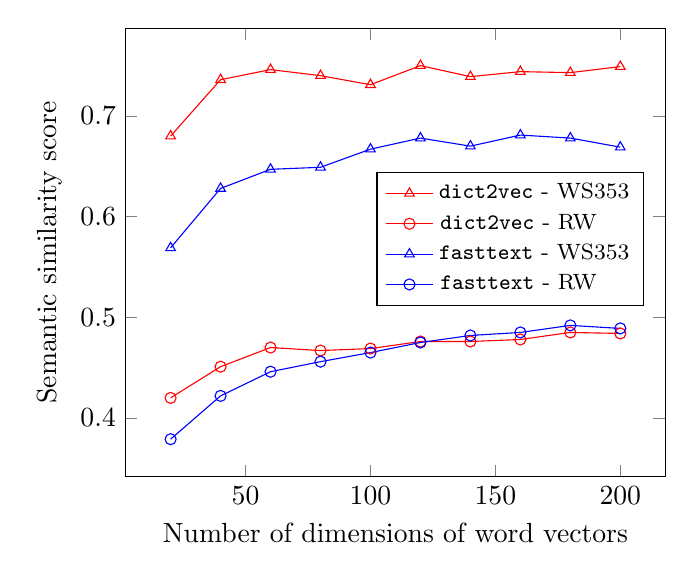
\begin{tikzpicture}
          \begin{axis}[
              xlabel=Number of dimensions of word vectors,
              ylabel=Semantic similarity score,
              legend style={at={(0.96,0.53)}, anchor=east, font=\footnotesize}]
            % fasttext in BLUE, dict2vec in RED
            % RW in circle, WSALL in triangle
            \addplot[color=red, mark=triangle] coordinates { % WS353-ALL - our
              (20,0.680)
              (40,0.736)
              (60,0.746)
              (80,0.740)
              (100,0.731)
              (120,0.750)
              (140,0.739)
              (160,0.744)
              (180,0.743)
              (200,0.749)
            };
            \addplot[color=red, mark=o] coordinates { % RW - our
              (20,0.420)
              (40,0.451)
              (60,0.470)
              (80,0.467)
              (100,0.469)
              (120,0.476)
              (140,0.476)
              (160,0.478)
              (180,0.485)
              (200,0.484)
            };
            \addplot[color=blue, mark=triangle] coordinates { % WS353-ALL - FT
              (20,0.569)
              (40,0.628)
              (60,0.647)
              (80,0.649)
              (100,0.667)
              (120,0.678)
              (140,0.670)
              (160,0.681)
              (180,0.678)
              (200,0.669)
            };
            \addplot[color=blue, mark=o] coordinates { % RW - FT
              (20,0.379)
              (40,0.422)
              (60,0.446)
              (80,0.456)
              (100,0.465)
              (120,0.475)
              (140,0.482)
              (160,0.485)
              (180,0.492)
              (200,0.489)
            };
            \legend{\texttt{dict2vec} - WS353, \texttt{dict2vec} - RW~~~~~,
                    \texttt{fasttext} - WS353, \texttt{fasttext} - RW~~~~~}
          \end{axis}
        \end{tikzpicture}
        \caption[Evolution of semantic similarity according to the size of word
        vectors.]{Semantic similarity scores on the RW and the WS353-ALL datasets
        for \texttt{fasttext} and \texttt{dict2vec} word embeddings trained with
        different numbers of dimensions on the ``Wikipedia'' corpus of 50M
        tokens.}
        \label{ch05:fig:dimensions-embeddings}
      \end{figure}

    \paragraph{Training time.}
      The source code of the \texttt{dict2vec} model is based on the source code
      of the \texttt{word2vec} model, but the majority of the code has been
      rewritten and optimized for a faster training of word embeddings. The
      training times of different models on different corpora sizes are reported
      in~\autoref{ch05:tab:training-times} (all experiments were run on a Intel
      E3-1246 v3 processor). Although \texttt{dict2vec} performs more operations
      during training than the \texttt{word2vec} Skip-gram model (because of the
      additional positive sampling and the controlled negative sampling), it is
      $4$ times faster due to its code optimizations for
      word embeddings learned from the full Wikipedia dump, and almost $3$ times
      as fast as \texttt{fasttext}.

      \begin{table}[h]
        \centering
        \begin{tabular}{lccc}
                            &  50M  & 200M & full \\
        \midrule
          \texttt{word2vec} & 15m30 & 86m  & 2600m \\
          \texttt{fasttext} & 8m44  & 66m  & 1870m \\
          \texttt{dict2vec} & 4m09  & 26m  & 642m \\
        \bottomrule
        \end{tabular}
        \caption[Training time of the \texttt{word2vec}, \texttt{fasttext} and
        \texttt{dict2vec} models.]{Training time (in minutes) of the
        \texttt{word2vec}, \texttt{fasttext} and \texttt{dict2vec} models for
        several corpora sizes.}
        \label{ch05:tab:training-times}
      \end{table}

\section{Conclusion}
  % description rapide de dict2vec modele
  This chapter presented the first contribution of this thesis. As pointed out
  in~\autoref{chap:methods-we}, most of the existing methods to learn word
  embeddings only use generic text corpora like Wikipedia. The model presented
  here, named \texttt{dict2vec}, uses additional information from lexical
  dictionaries during training to encode more linguistic and semantic
  information into word embeddings. It generates pairs of related words (and in
  some cases, pairs of strongly related words) based on the cooccurrences of
  terms in dictionary definitions and uses this additional information in a
  novel positive sampling to extend the \texttt{word2vec} model.\medskip

  % rappel des principaux resultats
  Word embeddings learned with \texttt{dict2vec} have largely improved results
  on a word semantic similarity task and are slightly better on a text
  classification task compared to other common methods used to learn word
  embeddings like \texttt{word2vec} or \texttt{fasttext}. Moreover,
  \texttt{dict2vec} is better than other methods which use external information
  to learn word embeddings like \texttt{retrofitting} or than methods which use
  WordNet as an additional source of knowledge because dictionaries contain
  stronger semantic information about words than WordNet. Further experiments
  have also demonstrated that simply adding definitions of words to a small
  training corpus is better than extending this small corpus with Wikipedia
  content: small but specific corpora are superior than large and generic ones,
  as the information contained in dictionaries is more refined and less
  noisy.\medskip

  % simplicity of dict2Vec + code used by people and on github
  One thing that has not been mentionned so far is the simplicity of the
  \texttt{dict2vec} model. Whether for creating strong and weak pairs or for
  learning word embeddings, all the computations and experiments of
  \texttt{dict2vec} have been able to run on the CPU of desktop computers. It
  was also possible to replicate the experiments from scratch on laptops, mainly
  due to the numerous code optimizations made from the original
  \texttt{word2vec} source code, leading to a faster and more efficient
  training. Source code to fetch dictionary definitions, generate related pairs
  of words, train the \texttt{dict2vec} model and evaluate the learned word
  embeddings on several datasets have been made publicly
  availabe\footnote{\url{https://github.com/tca19/dict2vec}}.\medskip

  % parler des gens qui nous etendent + piste amelioration
  Several works have extended the \texttt{dict2vec} model or the idea of using
  dictionaries to learn word embeddings.
  \citeauthor{bosc2018auto}~\citep{bosc2018auto} have proposed an architecture
  based on an autoencoder to learn a latent vector representation for each
  dictionary definition and reconstruct the definition from the latent vector.
  More recently, I participated in the development of an extension of the
  \texttt{dict2vec} model for the specific use case of anorexia detection. This
  system use pairs of words related to the semantic field of anorexia and update
  the word embeddings of these words to have more specific semantic information
  encoded into them. With the semantically-improved embeddings, a classifier
  system has better performances in a classification task which consists in
  detecting anorexia messages in social media posts. This work has been accepted
  and will appear in the proceedings of the IDA 2020
  conference~\citep{ramirez2020anorexia}. Another possible way to extend the
  \texttt{dict2vec} model is to consider the polysemy information. Indeed, when
  definitions are extracted from online dictionaries, all the definitions of a
  word are concatenated together without considering that a word can have
  different senses and therefore different definitions. By separating the
  definitions of different senses, it would be possible to learn one embedding
  per sense like in~\citep{iacobacci2015sensembed} to help downstream models to
  solve word sense disambiguation tasks~\citep{iacobacci2016embeddings}.
  \medskip

  % evoque la seconde contrib = reduire la taille en memoire
  Finally, although the \texttt{dict2vec} model is simple, the learned word
  embedding matrix can have a size in memory in the order of gigabytes, which is
  a problem for using vectors on low-resource devices. This raises a new
  question: how can we learn word vectors with the benefits of the additional
  knowledge of dictionaries captured by \texttt{dict2vec} but with a smaller
  memory size? \autoref{chap:methods-reduction} presented methods to reduce the
  size of representations and explained how changing the representation space to
  use integer vector values also has the advantage of speeding up vector
  operations. But most of the presented methods were not targeted at word
  embeddings for use in downstream models. The next chapter presents the second
  contribution of this thesis, which addresses the problem of reducing the memory
  size of word embeddings and making vector operations faster, especially for
  the computation of semantic similarities between word vectors in downstream
  models.
